\documentclass[10pt,aspectratio=169]{ntuabeamer}

\graphicspath{{assets/generated/}{assets/}}

\framesource{ho2020}{Ho, Jain, Abbeel. \emph{Denoising Diffusion Probabilistic Models}. NeurIPS, 2020.}
\framesource{song2021}{Song et al. \emph{Score-Based Generative Modeling through Stochastic Differential Equations}. ICLR, 2021.}
\framesource{lipman2023}{Lipman et al. \emph{Flow Matching for Generative Modeling}. ICLR, 2023.}
\framesource{liu2023}{Liu, Gong, Liu. \emph{Flow Straight and Fast: Learning to Generate and Transfer Data with Rectified Flow}. ICLR, 2023.}

\title{Diffusion Models and Flow Matching}
\subtitle{Discrete-time denoising, continuous transport, and exact visualization examples}
\author{NTUA School of Civil Engineering}
\date{\today}

\begin{document}

\begin{frame}[plain]
  \makepresentationtitle
\end{frame}

\sectiondivider{Diffusion Models}

\begin{frame}{Diffusion: Visual Idea\framecite{ho2020}}
  \scriptsize
  \[
    x_0 \rightarrow x_1 \rightarrow x_2 \rightarrow \cdots \rightarrow x_T
  \]

  \begin{figure}
    \centering
    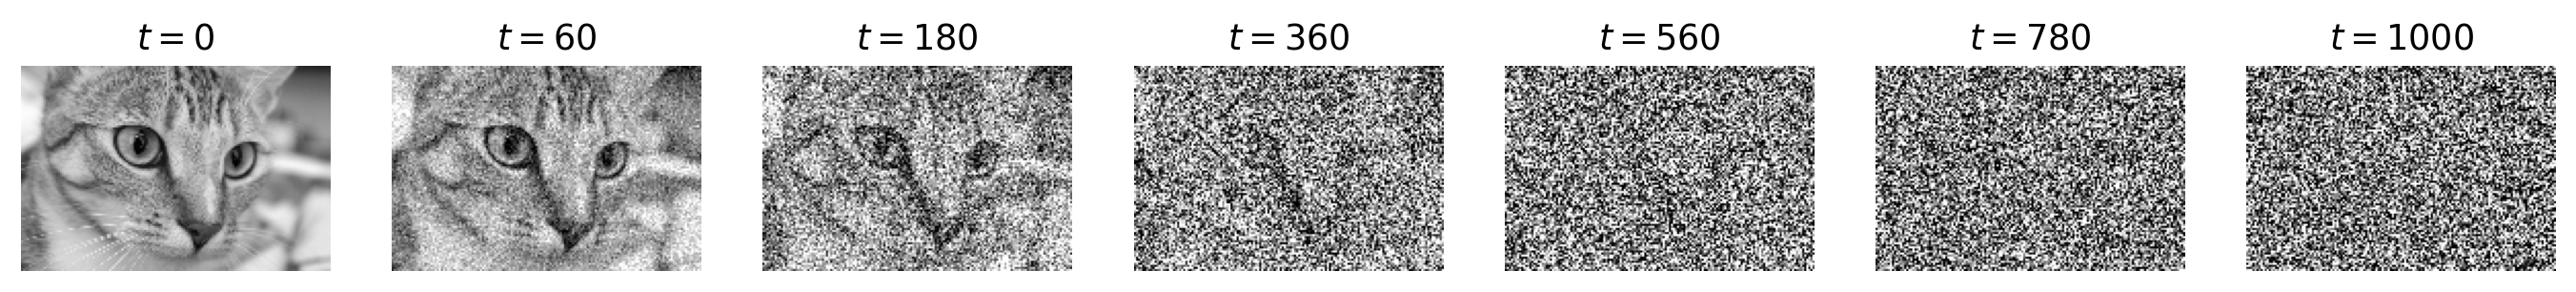
\includegraphics[width=\textwidth]{diffusion_forward_chain_cat.png}
    \caption{Forward chain: increasing \(t\) makes the state more random.}
  \end{figure}

  \[
    x_T \rightarrow x_{T-1} \rightarrow \cdots \rightarrow x_1 \rightarrow x_0
  \]

  \begin{figure}
    \centering
    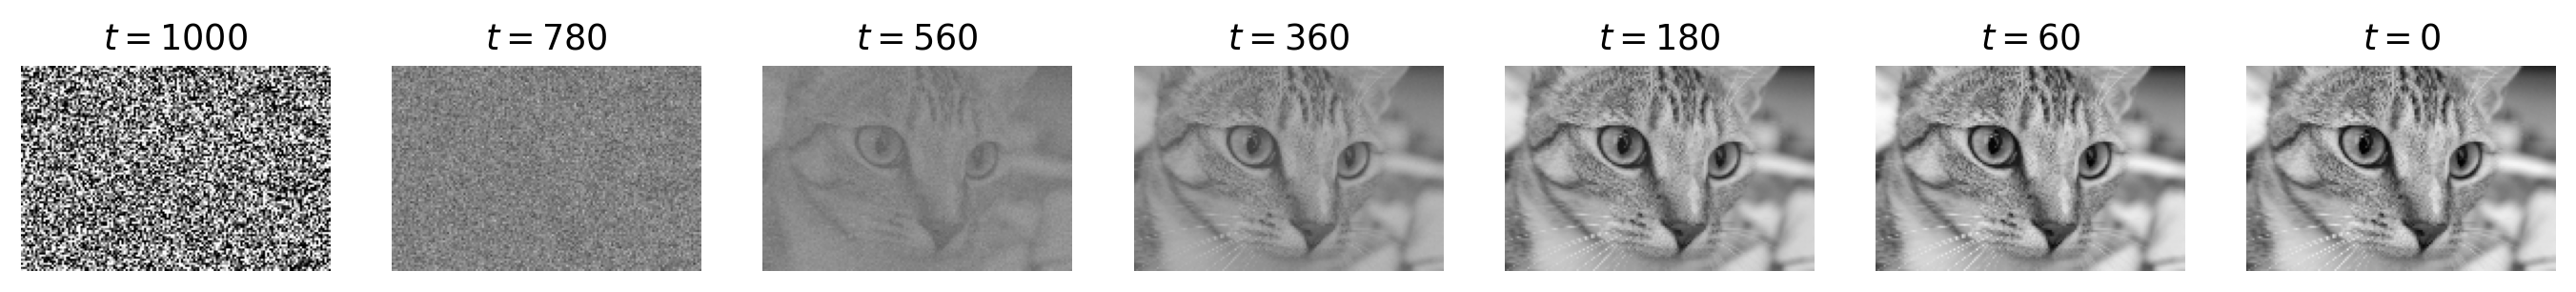
\includegraphics[width=\textwidth]{diffusion_reverse_chain_cat_oracle.png}
    \caption{Posterior-mean reverse chain from the same terminal noisy state \(x_T\).}
  \end{figure}
\end{frame}

\begin{frame}{Diffusion Notation}
  \small
  \begin{itemize}
    \item \(x_0\): clean data sample, \(x_t\): sample after \(t\) noising steps
    \item \(t \in \{1,\dots,T\}\), with \(x_T\) close to isotropic Gaussian noise
    \item \(\beta_t \in (0,1)\): variance schedule at step \(t\)
    \item \(\alpha_t = 1-\beta_t\), \(\bar{\alpha}_t = \prod_{s=1}^{t} \alpha_s\)
    \item \(s_t = \sqrt{\bar{\alpha}_t}\), \(\sigma_t = \sqrt{1-\bar{\alpha}_t}\)
    \item \(q(\cdot)\): forward noising distribution, \(I\): identity covariance matrix
  \end{itemize}

  \[
    q(x_t \mid x_{t-1}) = \mathcal N\!\left(\sqrt{\alpha_t}\,x_{t-1}, \beta_t I\right)
  \]

  \[
    q(x_t \mid x_0) = \mathcal N\!\left(\sqrt{\bar{\alpha}_t}\,x_0, (1-\bar{\alpha}_t)I\right)
  \]
\end{frame}

\begin{frame}{Diffusion: Local Intuition}
  \begin{itemize}
    \item At reverse time \(t\), the model sees a noisy sample \(x_t\)
    \item The local question is: what correction points from the current noisy state \(x_t\) toward a cleaner next state \(x_{t-1}\)?
    \item The key geometric object is the score of the noisy marginal density
  \end{itemize}

  \[
    \nabla_x \log p_t(x)
  \]

  \begin{itemize}
    \item \(p_t\) denotes the density of samples at noise level \(t\)
    \item The score points in the direction of steepest increase of \(\log p_t(x)\)
    \item In reverse sampling, \(x_t\) is the current state and \(x_{t-1}\) is the next, less noisy state
    \item This is the continuous geometric picture behind denoising
  \end{itemize}
\end{frame}

\begin{frame}{Forward Discretization}
  \begin{itemize}
    \item The forward process is a Gaussian Markov chain
    \item Each step keeps most of the previous signal and injects fresh Gaussian noise
  \end{itemize}

  \[
    q(x_t \mid x_{t-1})
    =
    \mathcal N\!\left(\sqrt{\alpha_t}\,x_{t-1}, \beta_t I\right)
  \]

  \[
    x_t
    =
    \sqrt{\alpha_t}\,x_{t-1}
    +
    \sqrt{\beta_t}\,\varepsilon_t
  \]

  \begin{itemize}
    \item \(\varepsilon_t \sim \mathcal N(0,I)\): fresh Gaussian perturbation at step \(t\)
    \item \(\alpha_t\): signal retention, \(\beta_t\): injected noise variance
  \end{itemize}
\end{frame}

\begin{frame}{Direct Noisy-Sample Formula}
  \begin{itemize}
    \item The closed form of \(q(x_t \mid x_0)\) lets us sample any noise level directly
  \end{itemize}

  \[
    x_t
    =
    \sqrt{\bar{\alpha}_t}\,x_0
    +
    \sqrt{1-\bar{\alpha}_t}\,\varepsilon
    =
    s_t x_0 + \sigma_t \varepsilon
  \]

  \begin{itemize}
    \item \(x_0\): clean image, \(x_t\): image at noise level \(t\)
    \item \(\varepsilon \sim \mathcal N(0,I)\): Gaussian noise used in the direct perturbation
    \item \(\bar{\alpha}_t\): accumulated signal retention
    \item \(s_t,\sigma_t\): shorthand signal and noise scales in the direct formula
  \end{itemize}
\end{frame}

\begin{frame}{Training Objective}
  \begin{itemize}
    \item The network receives a noisy sample \(x_t\) and the timestep \(t\)
    \item It predicts the Gaussian noise used in the closed-form perturbation
  \end{itemize}

  \[
    \min_\theta
    \mathbb E_{x_0,\varepsilon,t}
    \left[
      \left\|
        \varepsilon_\theta(x_t,t) - \varepsilon
      \right\|^2
    \right]
  \]

  \[
    x_t
    =
    \sqrt{\bar{\alpha}_t}\,x_0
    +
    \sqrt{1-\bar{\alpha}_t}\,\varepsilon
  \]

  \begin{itemize}
    \item \(\varepsilon_\theta(x_t,t)\): predicted noise, \(\theta\): learnable network parameters
    \item The expectation averages over clean data, sampled noise, and sampled timesteps
  \end{itemize}
\end{frame}

\begin{frame}{Why Noise Prediction Works}
  \small
  \begin{itemize}
    \item For the conditional Gaussian perturbation, the score is exact and explicit
  \end{itemize}

  \[
    \nabla_{x_t} \log q(x_t \mid x_0)
    =
    -\frac{x_t - \sqrt{\bar{\alpha}_t}\,x_0}{1-\bar{\alpha}_t}
  \]

  \begin{itemize}
    \item If \(x_t\) is far from the clean signal, the correction magnitude is large
    \item This identity is conditional on \(x_0\), so \(q(x_t\mid x_0)\) is the relevant density here
    \item The marginal score \(\nabla_x \log p_t(x)\) is obtained after averaging over the data distribution
  \end{itemize}
\end{frame}

\begin{frame}{Exact Score Field of a Smoothed Distribution}
  \begin{figure}
    \centering
    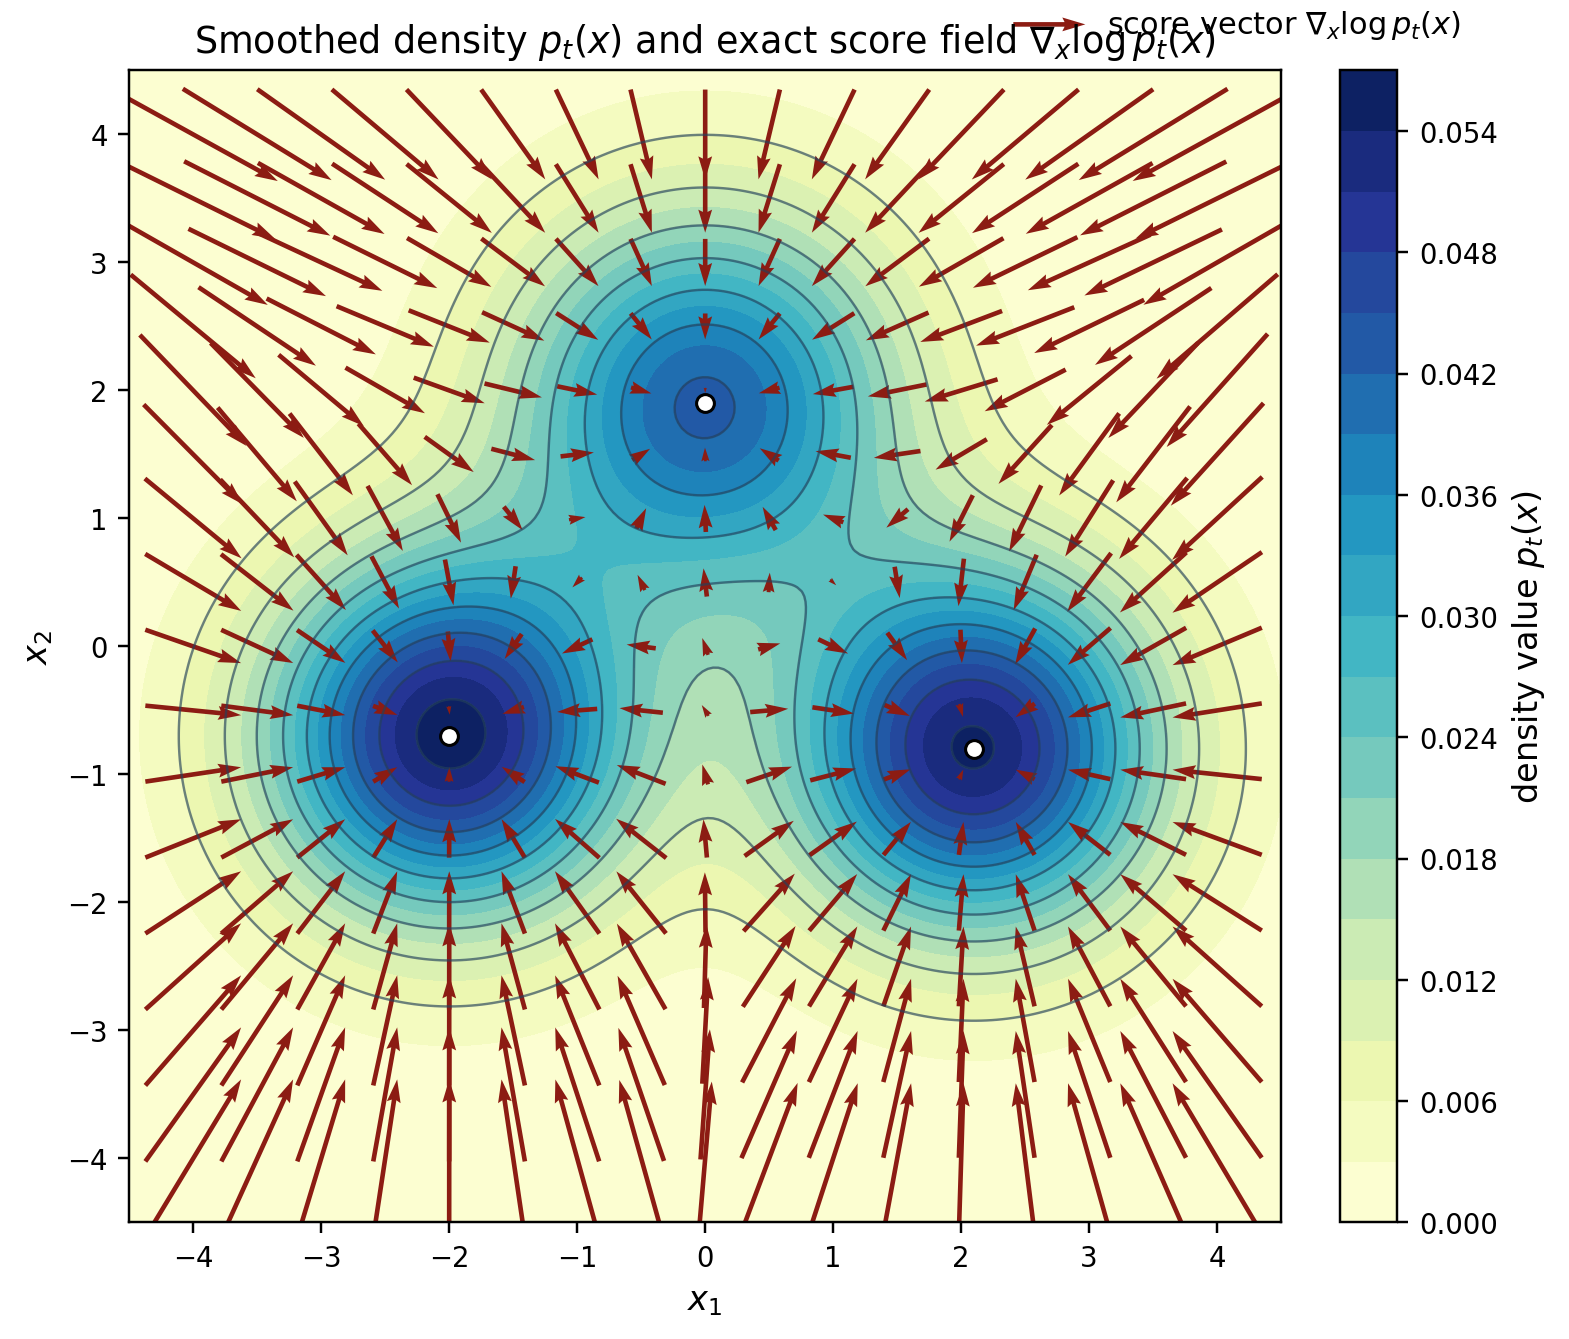
\includegraphics[height=0.59\textheight]{score_field_gaussian_mixture.png}
    \caption{Contours and color encode the smoothed density \(p_t(x)\). Arrows encode the exact score field \(\nabla_x \log p_t(x)\).}
  \end{figure}
\end{frame}

\begin{frame}{Reverse Process: Exact Posterior vs Learned Model}
  \small
  \begin{itemize}
    \item With access to \(x_0\), the forward model gives an exact reverse posterior
  \end{itemize}

  \[
    q(x_{t-1}\mid x_t, x_0)
    =
    \mathcal N\!\left(\mu_q(x_t,x_0), \tilde{\beta}_t I\right)
  \]

  \[
    \mu_q(x_t,x_0)
    =
    \frac{\sqrt{\bar{\alpha}_{t-1}}\beta_t}{1-\bar{\alpha}_t}x_0
    +
    \frac{\sqrt{\alpha_t}(1-\bar{\alpha}_{t-1})}{1-\bar{\alpha}_t}x_t
  \]

  \[
    \tilde{\beta}_t
    =
    \beta_t \frac{1-\bar{\alpha}_{t-1}}{1-\bar{\alpha}_t}
  \]

  \begin{itemize}
    \item \(\mu_q(x_t,x_0)\): exact posterior mean, \(\tilde{\beta}_t\): exact posterior variance coefficient
    \item \(p_\theta(x_{t-1}\mid x_t)\): learned reverse model used in practice
  \end{itemize}
\end{frame}

\begin{frame}{Diffusion: Algorithmic View}
  \small
  \twocols{%
    \textcolor{ntuablue}{Training}

    \begin{enumerate}
      \item Sample a clean data point \(x_0 \sim p_{\mathrm{data}}\)
      \item Sample a timestep \(t \in \{1,\dots,T\}\) and noise \(\varepsilon \sim \mathcal N(0,I)\)
      \item Form
        \[
          x_t=\sqrt{\bar{\alpha}_t}\,x_0+\sqrt{1-\bar{\alpha}_t}\,\varepsilon
        \]
      \item Predict \(\varepsilon_\theta(x_t,t)\)
      \item Update \(\theta\) to reduce
        \[
          \|\varepsilon_\theta(x_t,t)-\varepsilon\|^2
        \]
    \end{enumerate}
  }{%
    \textcolor{ntuablue}{Inference / Sampling}

    \begin{enumerate}
      \item Sample \(x_T \sim \mathcal N(0,I)\)
      \item For \(t=T,T-1,\dots,1\):
        \[
          \text{use } \varepsilon_\theta(x_t,t) \text{ to define } p_\theta(x_{t-1}\mid x_t)
        \]
      \item Sample or take the mean of \(x_{t-1}\) from that reverse model
      \item Repeat until reaching \(x_0\)
      \item Return the final denoised sample
    \end{enumerate}
  }
\end{frame}

\sectiondivider{Continuous Flows}

\begin{frame}{Continuous-Time Flow Idea}
  \begin{itemize}
    \item Start from a simple sample \(x_0\), typically Gaussian noise
    \item Move that point continuously toward the data distribution
    \item The model outputs a time-dependent velocity field
  \end{itemize}

  \[
    \frac{d x_t}{dt} = v_\theta(x_t,t),
    \qquad t \in [0,1]
  \]

  \begin{itemize}
    \item \(v_\theta(x_t,t)\): learned velocity at state \(x_t\) and time \(t\)
    \item Direction tells the sample where to move, magnitude tells it how fast to move
  \end{itemize}
\end{frame}

\begin{frame}{Flow Matching / Rectified Flow Path\framecite{lipman2023}\framecite{liu2023}}
  \begin{itemize}
    \item Sample a source point \(x_0\) and a target point \(x_1\)
    \item Connect them with a straight interpolation path
  \end{itemize}

  \[
    x_t = (1-t)x_0 + t x_1,
    \qquad t \in [0,1]
  \]

  \[
    \frac{d x_t}{dt} = x_1 - x_0
  \]

  \[
    u_t(x_t \mid x_0, x_1) = x_1 - x_0
  \]

  \begin{itemize}
    \item \(x_0\): source sample, \(x_1\): target sample
    \item \(u_t(x_t \mid x_0, x_1)\): pairwise target velocity for one sampled coupling pair
  \end{itemize}
\end{frame}

\begin{frame}{Flow Matching Objective}
  \small
  \begin{itemize}
    \item The target velocity is explicit for each sampled pair \((x_0, x_1)\)
    \item The network regresses from the interpolated point \(x_t\) and time \(t\) to that target
  \end{itemize}

  \[
    \min_\theta
    \mathbb E_{x_0,x_1,t}
    \left[
      \left\|
        v_\theta(x_t,t) - (x_1-x_0)
      \right\|^2
    \right]
  \]

  \begin{itemize}
    \item \(v_\theta(x_t,t)\): learned field, \(x_1-x_0\): pairwise target velocity for one coupling pair
    \item Important: \(x_1-x_0\) is not the same global vector field everywhere in state space
  \end{itemize}
\end{frame}

\begin{frame}{Flow Sampling Requires Numerical Integration}
  \small
  \begin{itemize}
    \item Continuous flows and flow matching define an ODE, not a closed-form final sample
    \item To generate \(x_1\) from \(x_0\), we must integrate
      \[
        \frac{d x_t}{dt} = v_\theta(x_t,t)
      \]
    \item Here \(x_t\) is the current state, \(t\) is time, and \(v_\theta(x_t,t)\) is the learned velocity field
  \end{itemize}

  \textcolor{ntuablue}{Euler step}
  \[
    x_{t+\Delta t}
    =
    x_t + \Delta t\, v_\theta(x_t,t)
  \]

  \textcolor{ntuablue}{Runge--Kutta midpoint step}
  \[
    k_1 = v_\theta(x_t,t), \qquad
    k_2 = v_\theta\!\left(x_t + \frac{\Delta t}{2}k_1,\ t+\frac{\Delta t}{2}\right)
  \]
  \[
    x_{t+\Delta t}
    =
    x_t + \Delta t\,k_2
  \]
\end{frame}

\begin{frame}{1D Transport Field Between Endpoint Distributions}
  \begin{figure}
    \centering
    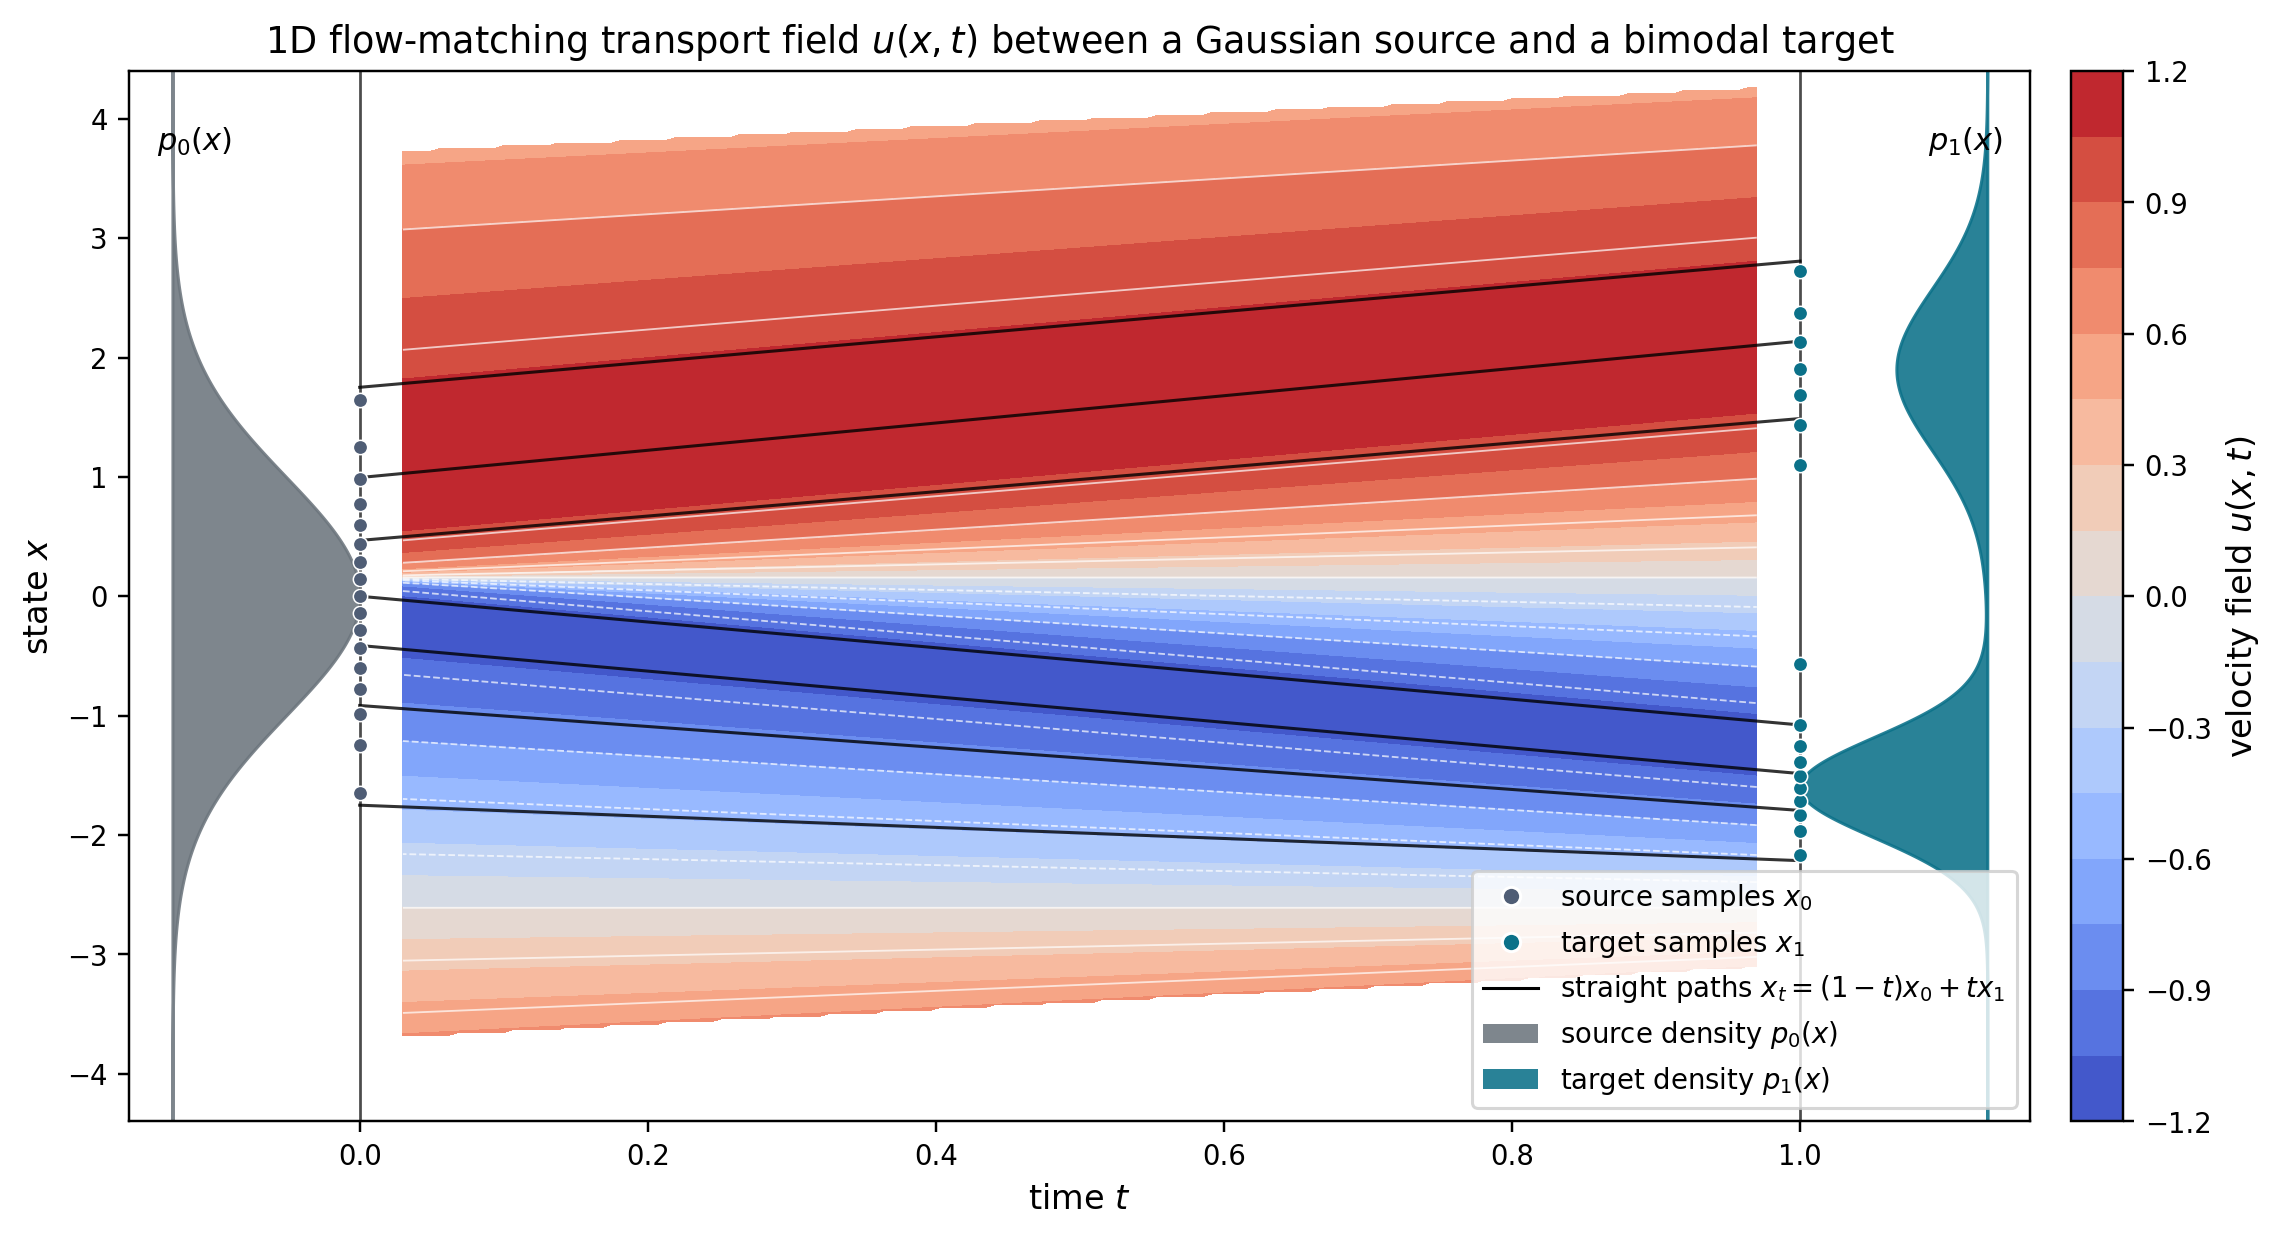
\includegraphics[height=0.59\textheight]{flow_matching_1d_transport_field.png}
    \caption{Gray points and band: source samples and density \(p_0(x)\). Blue points and band: target samples and density \(p_1(x)\). Black curves: straight paths \(x_t=(1-t)x_0+t x_1\). Middle contour: \(u(x,t)=\mathbb E[x_1-x_0 \mid x_t=x]\).}
  \end{figure}
\end{frame}

\begin{frame}{Flow Matching: Algorithmic View}
  \small
  \twocols{%
    \textcolor{ntuablue}{Training}

    \begin{enumerate}
      \item Sample a source point \(x_0 \sim p_0\) and a data point \(x_1 \sim p_1\)
      \item Sample a time \(t \sim \mathrm{Uniform}[0,1]\)
      \item Build the interpolated state
        \[
          x_t=(1-t)x_0+t x_1
        \]
      \item Form the pairwise target velocity
        \[
          u_t(x_t\mid x_0,x_1)=x_1-x_0
        \]
      \item Update \(\theta\) to reduce
        \[
          \|v_\theta(x_t,t)-(x_1-x_0)\|^2
        \]
    \end{enumerate}
  }{%
    \textcolor{ntuablue}{Inference / Sampling}

    \begin{enumerate}
      \item Sample an initial point \(x_0 \sim p_0\)
      \item Solve the ODE
        \[
          \frac{d x_t}{dt}=v_\theta(x_t,t), \qquad t\in[0,1]
        \]
      \item Use a numerical integrator such as Euler or midpoint Runge--Kutta
      \item March from \(t=0\) to \(t=1\)
      \item Return the transported point \(x_1\)
    \end{enumerate}
  }
\end{frame}

\sectiondivider{Comparison}

\begin{frame}{Diffusion vs Flow Matching}
  \twocols{%
    \textcolor{ntuablue}{Diffusion}

    \begin{itemize}
      \item Forward model corrupts data with Gaussian noise
      \item Training target is the added noise \(\varepsilon\)
      \item Reverse generation approximates repeated denoising steps
      \item Local geometric view uses the score \(\nabla_x \log p_t(x)\)
    \end{itemize}
  }{%
    \textcolor{ntuablue}{Flow Matching}

    \begin{itemize}
      \item Training constructs interpolation paths between source and target samples
      \item Training target is the pairwise conditional velocity \(x_1-x_0\)
      \item Generation solves an ODE driven by a learned velocity field
      \item Local geometric view uses the vector field \(v_\theta(x,t)\)
    \end{itemize}
  }
\end{frame}

\end{document}
